% Исследовательский раздел
\chapter{Исследовательский раздел}

\section{Описание исследования}

В исследовательском разделе проведено исследование для оценки времени выполнения ключевых операций разработанной базы данных медицинской клиники при увеличении объема данных. Исследование выполнялось на контейнерном стенде, включающем PostgreSQL, Redis, backend-приложение на Go и frontend-приложение на React.

Для проведения исследования использовался сценарий research\_benchmark.sql из каталога db. В отличие от вспомогательных проверок, данный сценарий не откатывает изменения, а наполняет рабочую базу данных исследовательским набором записей. Это позволяет проводить замеры на реально заполненных таблицах, которые затем доступны backend-приложению и frontend-интерфейсу.

В ходе исследования последовательно формировались три серии данных: 5000, 20000 и 50000 записей в основных таблицах предметной области. После каждой серии выполнялась команда ANALYZE. Для исследования влияния индексов и оптимизации SQL-запросов выполнялись замеры внутри PostgreSQL: для каждой операции проводилось семь запусков EXPLAIN ANALYZE. В таблицах и графиках приведено среднее время выполнения в миллисекундах. Redis-кэширование исследовалось отдельно как полное время HTTP-запроса к backend-приложению.

Измерялись следующие операции:
\begin{itemize}
    \item получение расписания врача за период с использованием индексов;
    \item получение расписания врача при отключенных index scan и bitmap scan;
    \item получение расписания врача через backend при последовательном добавлении индексов и Redis-кэширования;
    \item получение истории приемов пациента;
    \item получение счетов пациента;
    \item построение отчета по выручке врача;
    \item вставка новой записи на прием через функцию book\_appointment схемы scheduling;
    \item поиск строк по идентификатору пациента с индексом и без индекса на отдельной исследовательской таблице.
\end{itemize}

После завершения исследования база данных содержала строки, приведенные в таблице~\ref{tab:research-final-counts}.

\begin{table}[H]
    \centering
    \caption{Количество строк после выполнения исследовательского сценария}
    \label{tab:research-final-counts}
    \footnotesize
    \renewcommand{\arraystretch}{1.08}
    \begin{tabularx}{\textwidth}{|>{\raggedright\arraybackslash}p{7cm}|>{\centering\arraybackslash}X|}
        \hline
        Таблица & Количество строк \tabularnewline
        \hline
        medical.patients & 50002 \tabularnewline
        \hline
        scheduling.appointments & 50008 \tabularnewline
        \hline
        medical.visits & 50000 \tabularnewline
        \hline
        billing.invoices & 50000 \tabularnewline
        \hline
        billing.invoice\_items & 50000 \tabularnewline
        \hline
        billing.payments & 50000 \tabularnewline
        \hline
    \end{tabularx}
\end{table}
\normalsize

\section{Результаты исследования}

Результаты PostgreSQL-замеров приведены в таблице~\ref{tab:research-results}. Время измерялось в миллисекундах.

\begin{table}[H]
    \centering
    \caption{Среднее время выполнения операций}
    \label{tab:research-results}
    \scriptsize
    \renewcommand{\arraystretch}{1.08}
    \begin{tabularx}{\textwidth}{|>{\centering\arraybackslash}p{1.75cm}|>{\centering\arraybackslash}p{1.9cm}|>{\centering\arraybackslash}p{2.45cm}|>{\centering\arraybackslash}p{1.75cm}|>{\centering\arraybackslash}p{1.65cm}|>{\centering\arraybackslash}p{1.65cm}|>{\centering\arraybackslash}X|}
        \hline
        Объем & Расписание & Расписание без index scan & История пациента & Счета пациента & Отчет & Запись \tabularnewline
        \hline
        5000 & 1,717 & 1,745 & 0,176 & 0,129 & 4,828 & 0,559 \tabularnewline
        \hline
        20000 & 3,387 & 6,292 & 0,194 & 0,403 & 19,865 & 0,253 \tabularnewline
        \hline
        50000 & 7,614 & 23,188 & 0,143 & 1,325 & 57,672 & 0,276 \tabularnewline
        \hline
    \end{tabularx}
\end{table}
\normalsize

График времени выполнения операций чтения приведен на рисунке~\ref{fig:research-read-operations}.

\begin{figure}[H]
    \centering
    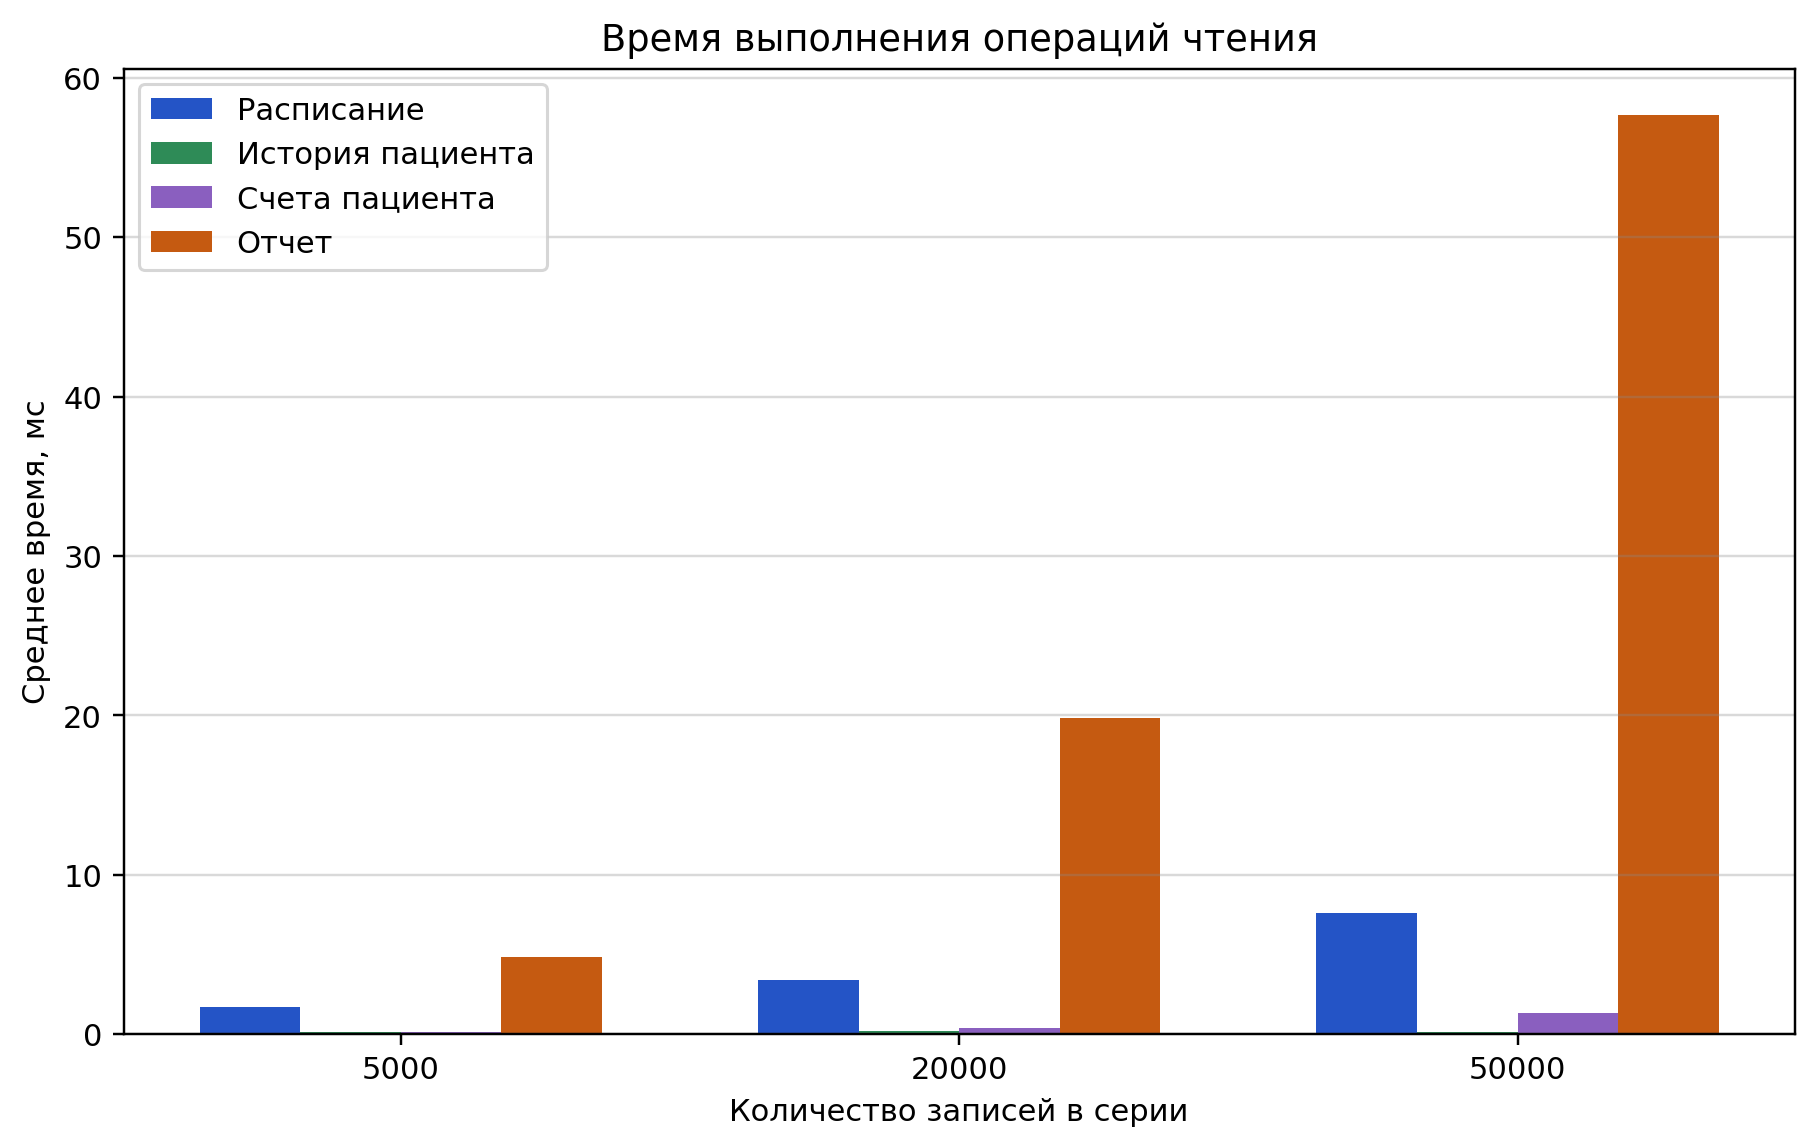
\includegraphics[width=0.95\textwidth]{figures/research_read_operations.png}
    \caption{Время выполнения операций чтения при разном объеме данных}
    \label{fig:research-read-operations}
\end{figure}

На рисунке~\ref{fig:research-index-impact} показано сравнение получения расписания врача при обычном плане выполнения и при отключенных index scan и bitmap scan.

\begin{figure}[H]
    \centering
    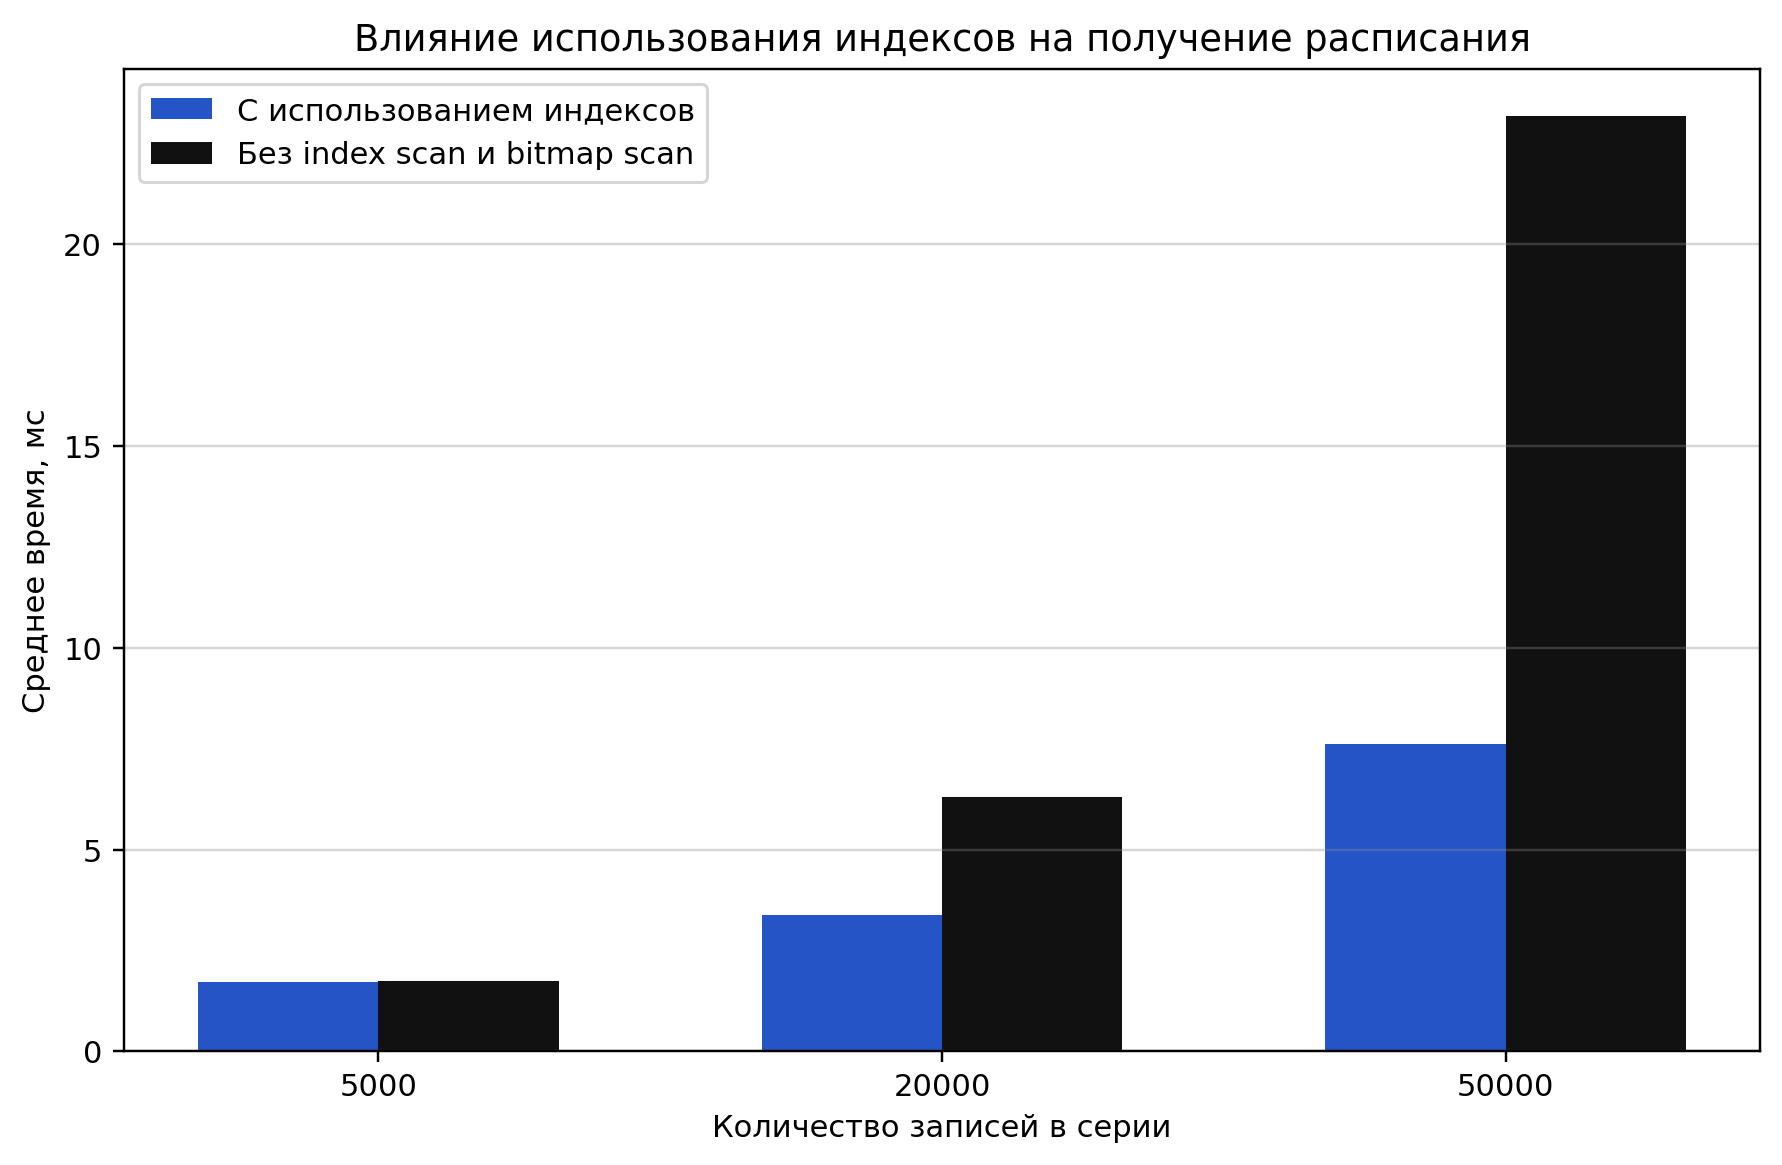
\includegraphics[width=0.9\textwidth]{figures/research_index_impact.png}
    \caption{Влияние использования индексов на получение расписания врача}
    \label{fig:research-index-impact}
\end{figure}

Дополнительно были выполнены замеры последовательного ускорения получения расписания врача на уровне полного HTTP-запроса к backend-приложению. Такой замер позволяет сравнить не только время выполнения SQL-запроса внутри PostgreSQL, но и полный путь пользовательского запроса: HTTP-обработку, обращение к базе данных или Redis, сериализацию JSON и передачу ответа.

Для каждого объема данных сравнивались три режима: запрос без Redis-кэша и без обычных B-tree индексов расписания, запрос без Redis-кэша при наличии индексов и повторный запрос из Redis-кэша. Перед запросами без Redis выполнялась очистка ключей Redis, чтобы backend был вынужден читать данные из PostgreSQL. Для режима без индексов временно удалялись индексы \texttt{idx\_schedule\_availability\_lookup}, \texttt{idx\_schedule\_absence\_lookup} и \texttt{idx\_appointments\_doctor\_time}; после замеров индексы создавались обратно. Для каждого режима усреднялись семь запусков. Результаты приведены в таблице~\ref{tab:research-http-schedule-chain}.

\begin{table}[H]
    \centering
    \caption{Ускорение полного HTTP-запроса расписания врача}
    \label{tab:research-http-schedule-chain}
    \scriptsize
    \renewcommand{\arraystretch}{1.08}
    \begin{tabularx}{\textwidth}{|>{\centering\arraybackslash}p{1.25cm}|>{\centering\arraybackslash}p{1.7cm}|>{\centering\arraybackslash}p{1.7cm}|>{\centering\arraybackslash}p{1.7cm}|>{\centering\arraybackslash}p{1.55cm}|>{\centering\arraybackslash}p{1.35cm}|>{\centering\arraybackslash}X|}
        \hline
        Объем & Без инд., мс & С инд., мс & Redis hit, мс & Индексы, \% & Redis, \% & Итог, \% \tabularnewline
        \hline
        5000 & 36,893 & 29,719 & 26,801 & 19,44 & 9,82 & 27,35 \tabularnewline
        \hline
        20000 & 149,756 & 105,388 & 97,442 & 29,63 & 7,54 & 34,93 \tabularnewline
        \hline
        50000 & 292,108 & 279,806 & 260,563 & 4,21 & 6,88 & 10,80 \tabularnewline
        \hline
    \end{tabularx}
\end{table}
\normalsize

На рисунке~\ref{fig:research-http-schedule-chain} показана цепочка ускорения полного HTTP-запроса: сначала за счет индексов PostgreSQL, затем за счет Redis-кэширования повторного запроса.

\begin{figure}[H]
    \centering
    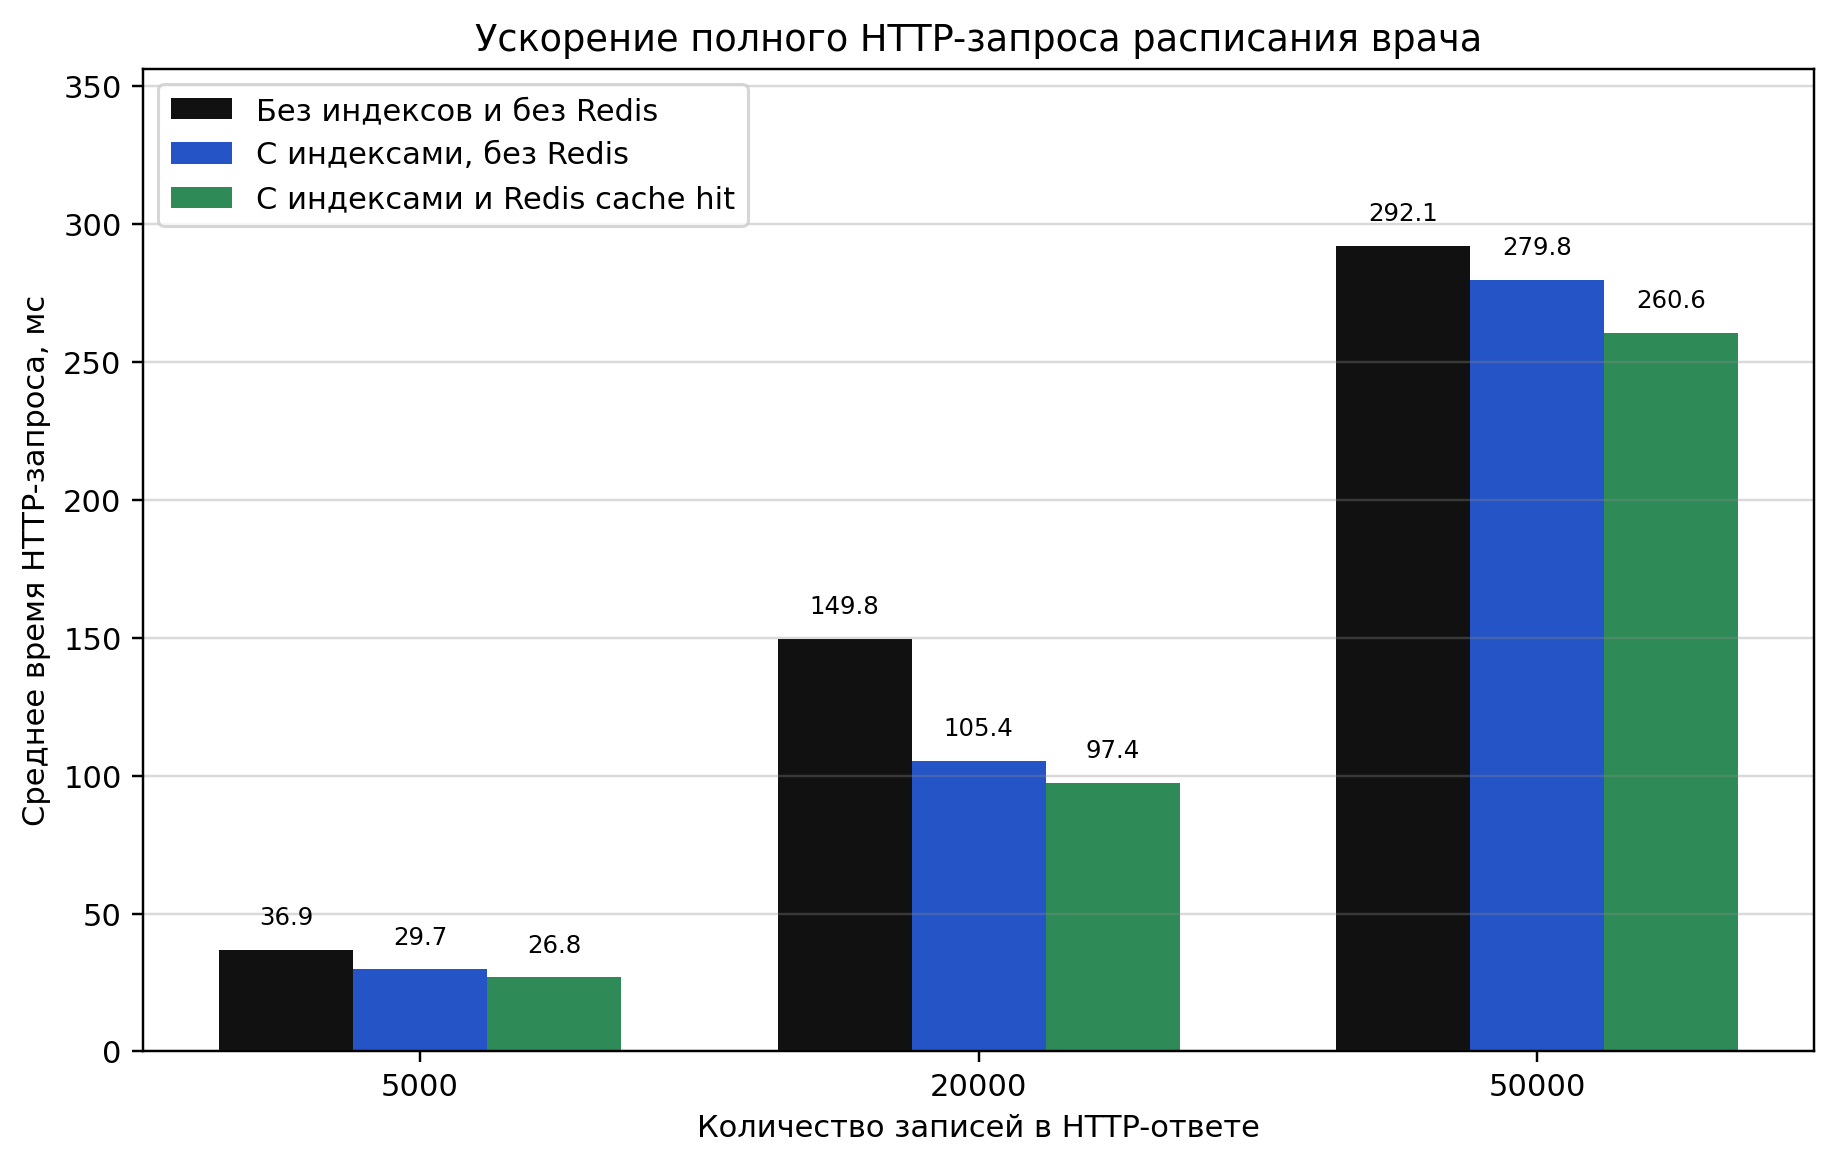
\includegraphics[width=0.9\textwidth]{figures/research_http_schedule_chain.png}
    \caption{Ускорение полного HTTP-запроса расписания врача}
    \label{fig:research-http-schedule-chain}
\end{figure}

График времени вставки новой записи на прием приведен на рисунке~\ref{fig:research-book-appointment}.

\begin{figure}[H]
    \centering
    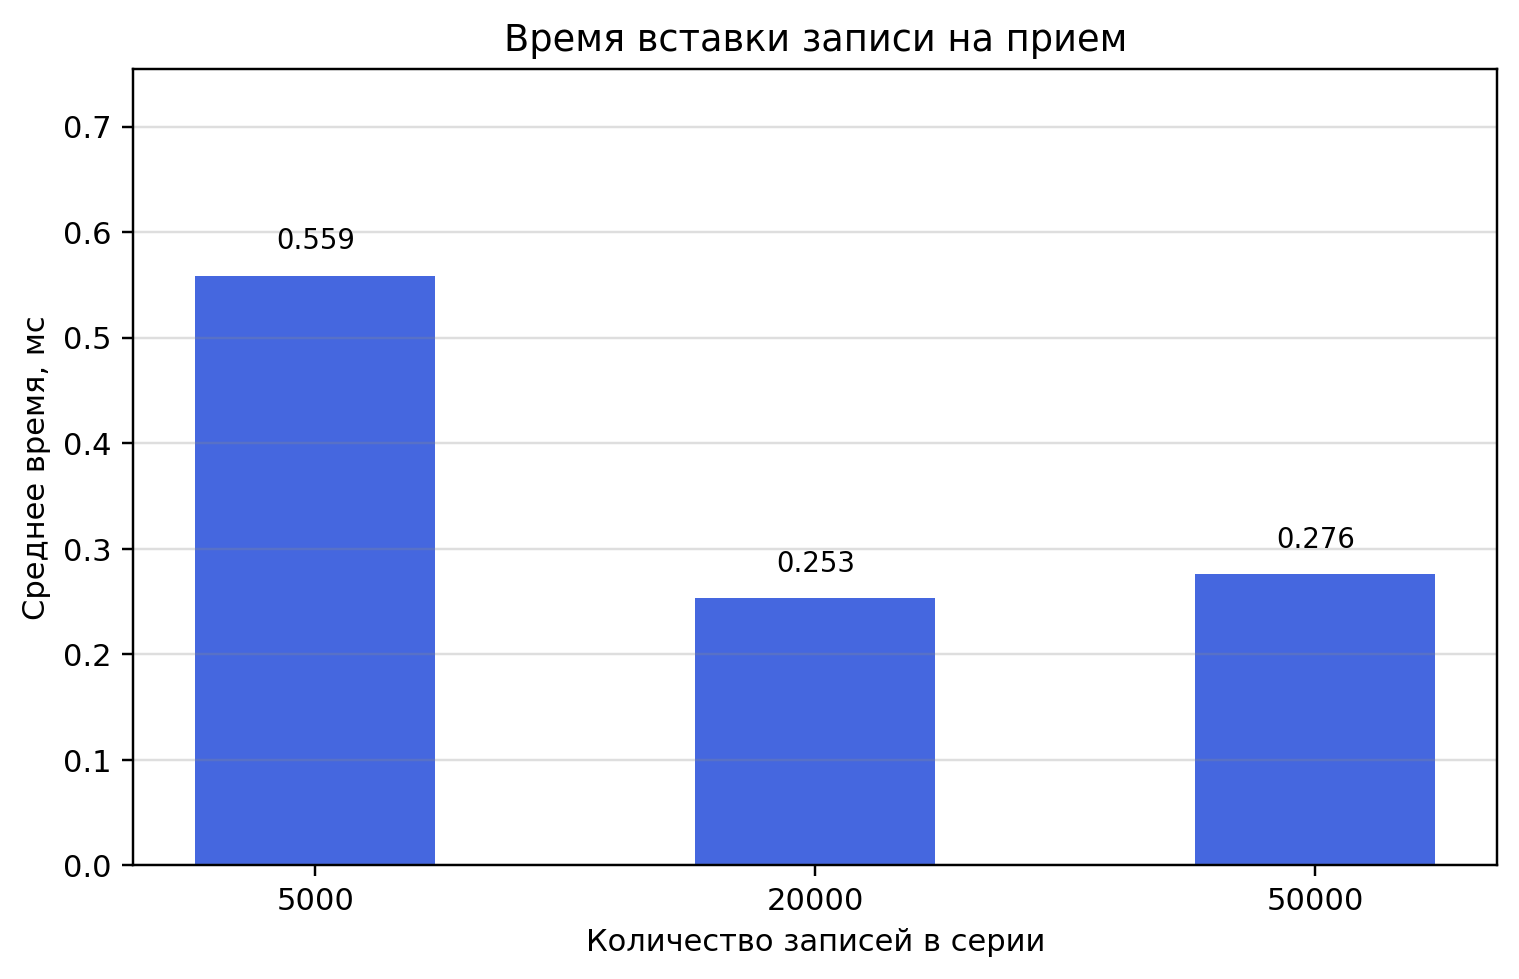
\includegraphics[width=0.86\textwidth]{figures/research_book_appointment.png}
    \caption{Время вставки записи на прием при разном объеме данных}
    \label{fig:research-book-appointment}
\end{figure}

Дополнительное исследование влияния индекса на поиск строк по идентификатору пациента приведено на рисунке~\ref{fig:research-index-search-piecewise}. Для него использовалась отдельная таблица \texttt{research\_index\_search}, которая последовательно наполнялась наборами от 1000 до 50000 строк. После каждого наполнения сравнивалось выполнение запроса без индекса и с B-tree индексом по полю \texttt{patient\_id}; для каждой точки усреднялись пять запусков EXPLAIN ANALYZE.

\begin{figure}[H]
    \centering
    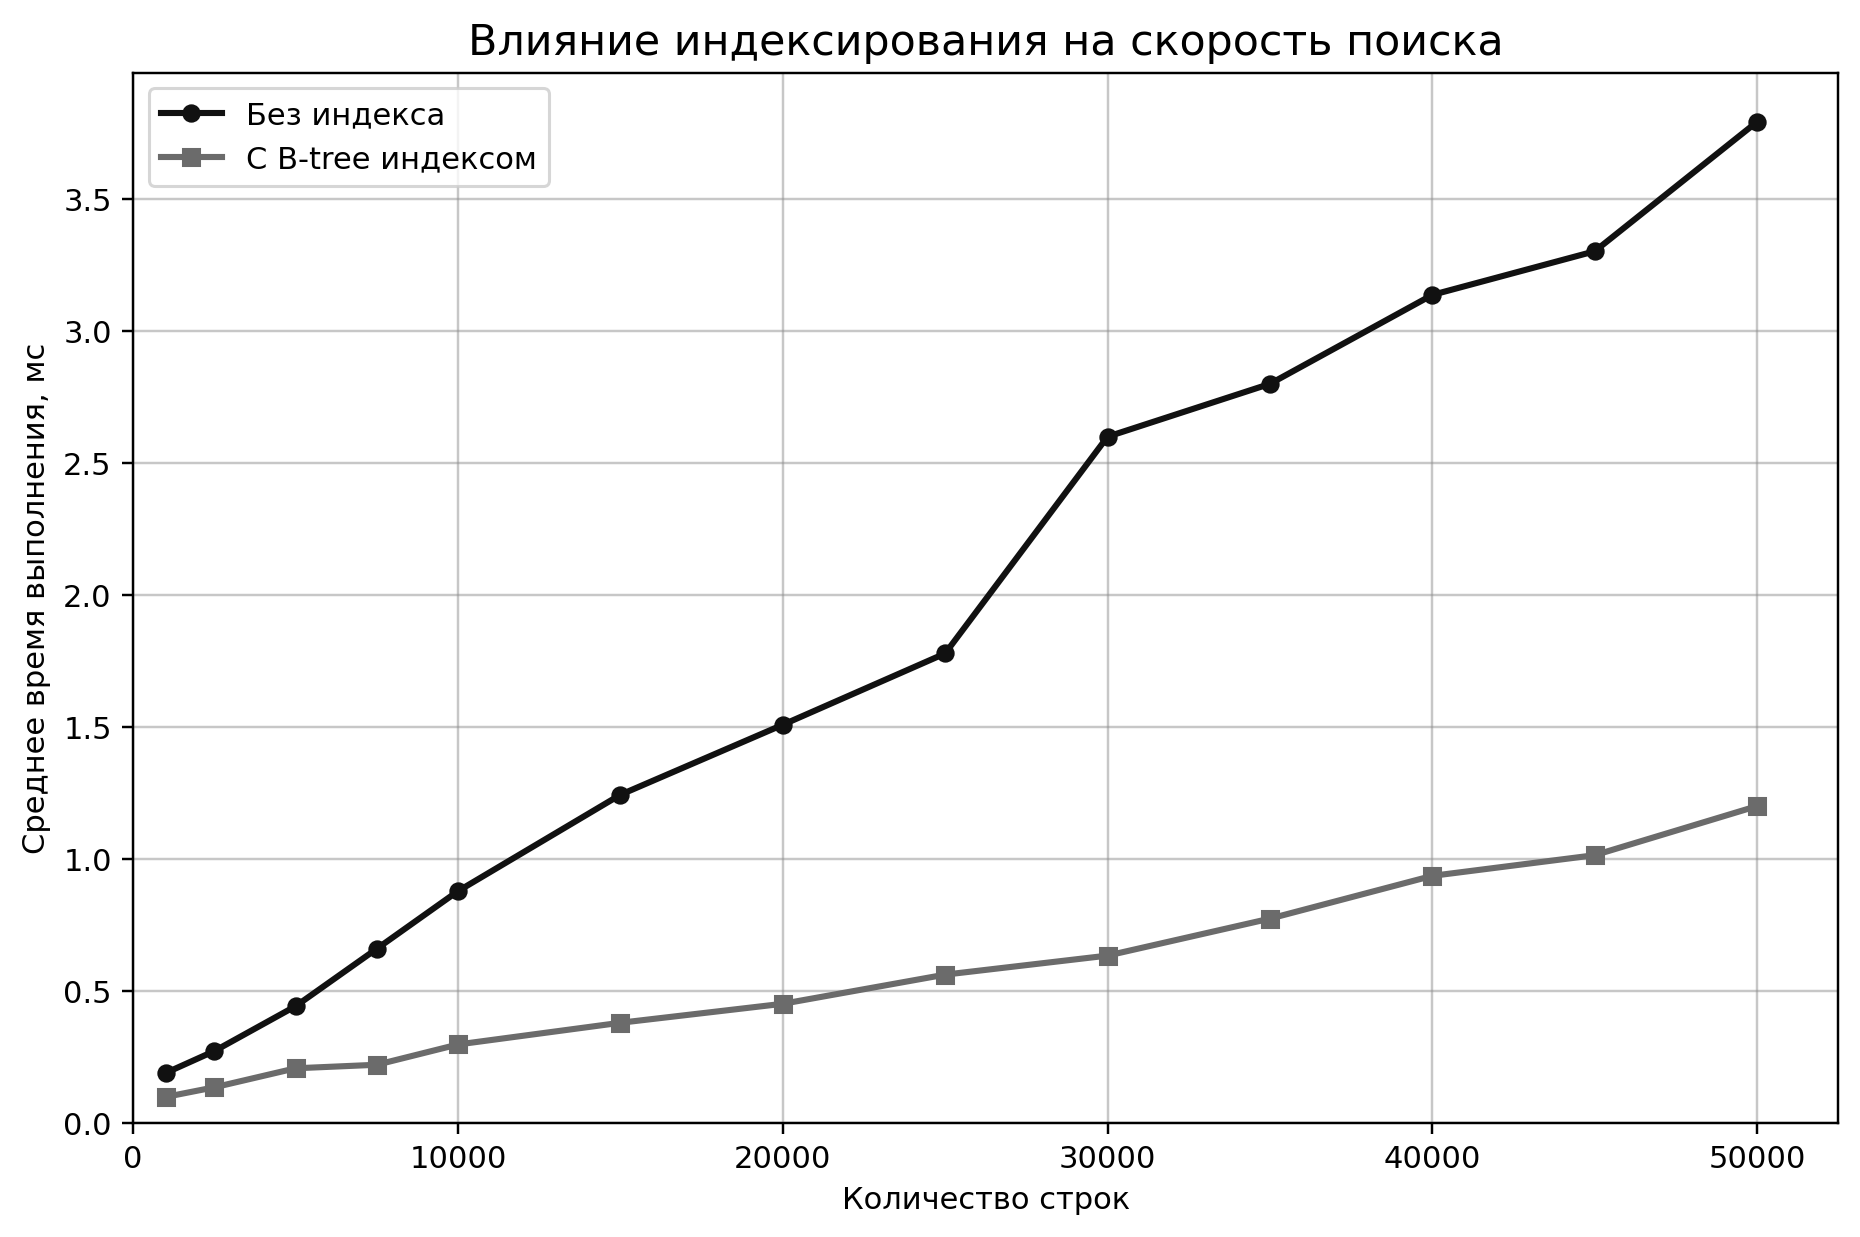
\includegraphics[width=0.9\textwidth]{figures/research_index_search_piecewise.png}
    \caption{Влияние индексирования на поиск по идентификатору пациента}
    \label{fig:research-index-search-piecewise}
\end{figure}

\section{Анализ результатов}

Наибольшее время выполнения показал отчет по выручке врача. При увеличении объема данных с 5000 до 50000 записей среднее время построения отчета выросло с 4,828 мс до 57,672 мс. Это объясняется тем, что запрос соединяет таблицы записей, приемов и счетов, после чего выполняет группировку результата.

Получение расписания врача при использовании индексов заняло 7,614 мс на объеме 50000 записей. При отключенных index scan и bitmap scan время той же операции выросло до 23,188 мс. Таким образом, на максимальном исследованном объеме использование индексов ускорило получение расписания примерно в 3 раза.

Дополнительный HTTP-замер показывает последовательный эффект оптимизаций на уровне всего backend-запроса. На объеме 20000 записей добавление индексов уменьшило среднее время с 149,756 мс до 105,388 мс, то есть на 29,63\%. Повторное чтение из Redis-кэша уменьшило время до 97,442 мс. На объеме 50000 записей итоговый выигрыш составил 10,80\%: время снизилось с 292,108 мс до 260,563 мс. Меньший выигрыш на максимальном объеме связан с тем, что существенную часть полного HTTP-запроса занимает не только доступ к PostgreSQL, но и сериализация, десериализация и передача большого JSON-ответа.

Запрос истории пациента и запрос счетов пациента выполнялись быстрее агрегирующего отчета. Для истории пациента среднее время на максимальном объеме составило 0,143 мс, для счетов пациента --- 1,325 мс. Это связано с тем, что данные запросы используют условия по patient\_id и ограничение количества возвращаемых строк.

Вставка записи через функцию scheduling.book\_appointment оставалась устойчивой на всех исследованных объемах. На 50000 записей среднее время составило 0,276 мс. Небольшая немонотонность значений связана с тем, что измерения выполняются на долях миллисекунды и зависят от состояния кэша PostgreSQL и планировщика контейнера. Кроме того, функция не просматривает всю таблицу записей, а выполняет проверки активности пациента, врача, услуги, доступности врача и отсутствия пересечения по времени с опорой на индексы и ограничение EXCLUDE.

Дополнительный график поиска по \texttt{patient\_id} показывает, что при росте числа строк запрос без индекса становится заметно медленнее, тогда как запрос с B-tree индексом растет значительно слабее. На объеме 50000 строк среднее время поиска без индекса составило 3,792 мс, а с индексом --- 1,201 мс.

\section{Вывод}

В результате исследования установлено, что разработанная структура базы данных сохраняет приемлемое время выполнения ключевых операций на объеме 50000 записей в основных таблицах. Наиболее чувствительной к росту объема данных является операция построения отчета по выручке, так как она требует соединения и агрегации большого числа строк.

Использование индексов существенно влияет на операции расписания: при 50000 записей отключение index scan увеличило время получения расписания с 7,614 мс до 23,188 мс. Дополнительный замер поиска по \texttt{patient\_id} также показал преимущество индексированного доступа. Операция записи пациента на прием через функцию базы данных осталась в пределах 0,276 мс на максимальном объеме, что подтверждает корректность выбранной стратегии согласованности: транзакционная функция PostgreSQL, индексы и EXCLUDE-ограничение позволяют предотвращать конфликтующие записи без существенного роста времени вставки.

Дополнительное исследование полного HTTP-запроса показало, что последовательное добавление индексов и Redis-кэширования уменьшает время получения расписания врача. При этом величина выигрыша зависит от размера ответа: на больших объемах данных ограничивающим фактором становится не только доступ к PostgreSQL, но и сериализация результата. Поэтому Redis целесообразно использовать для часто повторяющихся запросов расписания и прайс-листа, а также совместно с ограничением размера возвращаемого периода.

\clearpage
